\documentclass[11 pt]{article}

\usepackage{amsfonts}
\usepackage{amsmath}
\usepackage{fancyhdr}
\usepackage[left=2cm,right=2cm,top=2cm,bottom=2cm]{geometry}
\usepackage{graphicx}
\usepackage[hidelinks]{hyperref}
\usepackage{listings}
\usepackage{subfig}
\usepackage{xcolor}

\pagestyle{fancy}
\fancyhf{}
\lhead{Theoretical Statistical Physics}
\chead{Exercise 08}
\rhead{E. Dizer, V. Mader}
\setlength{\headheight}{15pt}

\newcommand{\pder}[2]{\frac{\partial #1}{\partial #2}} % total derivative
\newcommand{\tder}[2]{\frac{\dd #1}{\dd #2}} % partial derivative
\newcommand{\dd}{\mathrm{d}}
\newcommand{\red}[1]{\textcolor{red}{#1}} 
\newcommand{\blue}[1]{\textcolor{blue}{#1}} 
\newcommand{\green}[1]{\textcolor{green}{#1}} 

\definecolor{commentsColor}{rgb}{0.497495, 0.497587, 0.497464}
\definecolor{keywordsColor}{rgb}{0.000000, 0.000000, 0.635294}
\definecolor{stringColor}{rgb}{0.558215, 0.000000, 0.135316}
\lstnewenvironment{code}[2][]{%
    \lstset{ %
        backgroundcolor=\color{white},   % choose the background color; you must add \usepackage{color} or \usepackage{xcolor}
        basicstyle=\footnotesize,        % the size of the fonts that are used for the code
        breakatwhitespace=false,         % sets if automatic breaks should only happen at whitespace
        breaklines=true,                 % sets automatic line breaking
        % captionpos=b,                    % sets the caption-position to bottom
        commentstyle=\color{commentsColor}\textit,    % comment style
        deletekeywords={...},            % if you want to delete keywords from the given language
        escapeinside={\%*}{*)},          % if you want to add LaTeX within your code
        extendedchars=true,              % lets you use non-ASCII characters; for 8-bits encodings only, does not work with UTF-8
        frame=tb,	                   	   % adds a frame around the code
        keepspaces=true,                 % keeps spaces in text, useful for keeping indentation of code (possibly needs columns=flexible)
        keywordstyle=\color{keywordsColor}\bfseries,       % keyword style
        language=Python,                 % the language of the code (can be overrided per snippet)
        otherkeywords={*,...},           % if you want to add more keywords to the set
        numbers=left,                    % where to put the line-numbers; possible values are (none, left, right)
        numbersep=5pt,                   % how far the line-numbers are from the code
        numberstyle=\tiny\color{commentsColor}, % the style that is used for the line-numbers
        rulecolor=\color{black},         % if not set, the frame-color may be changed on line-breaks within not-black text (e.g. comments (green here))
        showspaces=false,                % show spaces everywhere adding particular underscores; it overrides 'showstringspaces'
        showstringspaces=false,          % underline spaces within strings only
        showtabs=false,                  % show tabs within strings adding particular underscores
        stepnumber=1,                    % the step between two line-numbers. If it's 1, each line will be numbered
        stringstyle=\color{stringColor}, % string literal style
        % tabsize=2,	                   % sets default tabsize to 2 spaces
        title=#2,                  % show the filename of files included with \lstinputlisting; also try caption instead of title
        columns=fixed                    % Using fixed column width (for e.g. nice alignment)
    }%
}{}


\begin{document}

    \section{
        Electrons in a metal as an ideal Fermi gas \textit{(7 points)}
    }
    As a classical model for paramagnetism one 
can consider a system of $N$ particles with 
the Hamiltonian
\begin{equation}
    \mathcal{H}=-hM
    \ \ \ \textnormal{with}\ \ \ 
    M=\mu\cdot\sum_{i=1}^N\cos\theta_i
\end{equation}
where $h$ is an external homogeneous magnetic 
field, $\mu$ the magnetic moment of a single 
particle and $\theta_i$ the angle between the
magnetic field $h$ and the magnetic moment
$\mu$ of particle $i$.

\paragraph{1. Use the canonical distribution 
    to calculate the average magnetization, 
    $\langle M\rangle$, as a function of $h$
    and temperature $T$. 
    \textit{(3 points)}
} \ \\
    \\
    Partition function:
    \begin{align}
        Z
        &=\frac{1}{h^{3N}}\cdot
        \int d^{3N}r 
        \int d^{3N}p
        \int d^N\Omega\
        e^{-\beta\mathcal{H}} \\
        &=Z_0\cdot\bigg(
            \int_0^{2\pi}d\varphi 
            \int_0^\pi d\theta
            \cdot\sin\theta\cdot 
            e^{h\beta\mu\sum_i^N\cos\theta_i}
        \bigg) \\
        &=Z_0\cdot\bigg(
            \int_0^{2\pi}d\varphi 
            \int_0^\pi d\theta
            \cdot\sin\theta\cdot 
            e^{h\beta\mu\cos\theta}
    \bigg)^N \\
        &=Z_0\cdot\bigg(
            \frac{4\pi\cdot\sinh(\beta\mu h)}
            {\beta\mu h}
        \bigg)^N
    \end{align}
    Free energy:
    \begin{align}
        F
        &=-k_BT\ln(Z) \\
        &=-k_BT\cdot(\ln(Z_0)+N\ln(4\pi))
        -Nk_BT\ln\bigg(
            \frac{\sinh(\beta\mu h)}{\beta\mu h}
        \bigg)
    \end{align}
    Magnetization:
    \begin{align}
        M
        =-\pder{F}{h}\bigg|_{T,V,N}
        =N\mu\cdot\bigg(\coth(x)
        -\frac{1}{x}\bigg)
    \end{align}
    with $x=\beta\mu h$.

\newpage
\paragraph{2. The ratio of which quantities 
    determines the average magnetization? 
    Sketch the functional dependence of the 
    average magnetization on this ratio. 
    \textit{(1 point)}
} \ \\
    \\
    The average magnetization is determined by 
    the ratio $\beta\mu h=\mu h/k_BT$.

    \begin{figure}[h!]
        \centering
        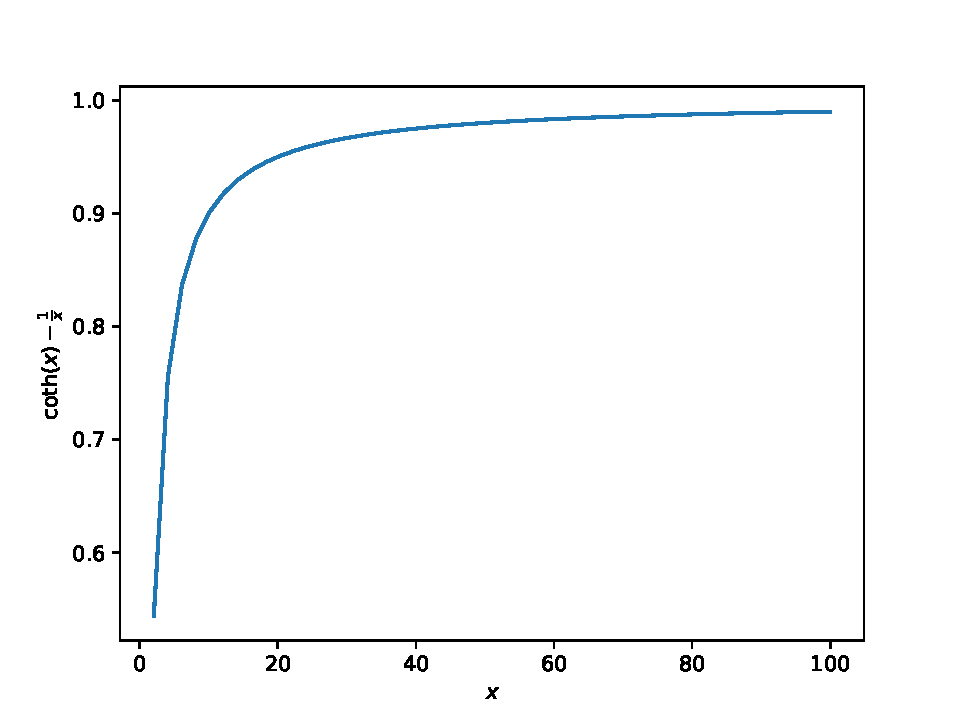
\includegraphics[width=.6\textwidth]{./figures/magnetization.pdf}
    \end{figure} \ \\ 

\paragraph{3. Discuss the two limiting cases: 
    high temperature/weak field vs. 
    low temperature/strong field.
    \textit{(2 points)}
} \ \\
    \\
    For $T\to0, M\sim N\mu$. \\
    For $T\to\infty, M\sim\frac{1}{2}N\mu(\beta\mu h)=\frac{1}{2}N\beta\mu^2 h\to0$

    \newpage

    \section{Particle-hole symmetry for fermions \textit{(4 points)}}
    Add this after tutorial!
    \newpage

    \section{Ultra-relativistic ideal Fermi fluid \textit{(4 points)}}
    In the lecture we have derived the following 
RG flow equation for the coupling constant $K$ 
of the Ising chain without magnetic field: 
the new value $K'$ is given by
\begin{equation}
    K'(K)=\frac{1}{2}\ln\cosh(2K).
\end{equation}
In addition we have derived the absolute 
increase in free energy per spin arising in 
each iteration:
\begin{equation}
    g(K)=\frac{1}{2}\ln2
    +\frac{1}{4}\ln\cosh(2K)
\end{equation}

\paragraph{1. Write a short computer program 
    (e.g. in Mathematica or Python) that 
    defines the flow equation $K'(K)$ and the 
    free energy increase $g(K)$ as functions. 
    Start with a coupling constant $K_0=1$ and 
    iterate through $K_1$, $K_2$, $K_3$ up to 
    $K_4$. Also calculated the corresponding 
    values $g_0=g(K_0)$ to $g_4=g(K_4).$ What 
    are the limits for these two series? 
    \textit{(1.5 points)}
} \ \\
    \\
    Python functions:
    \lstinputlisting[firstline=6, lastline=11]{./code/task03a.py}
    Iteration to $i=4$ yields
    \begin{table}[h!]
        \begin{center}
        \begin{tabular}{llllll}
                  & i=0  & i=1  & i=2  & i=3  & i=4  \\ 
            \hline
            $K_i$ & 1    & 0.66 & 0.35 & 0.11 & 0.01 \\ 
            $g_i$ & 0.68 & 0.52 & 0.4  & 0.35 & 0.35 \\ 
        \end{tabular}
        \end{center}
    \end{table} \ \\ 
    The $K_i$-series converges to zero for 
    large $i$, while the $g_i$-series 
    converges to $\frac{1}{2}\ln2\approx0.35$.
    \begin{figure}[h!]
        \centering
        \begin{minipage}{.5\linewidth}
          \centering
          \subfloat[coupling constant $K$]{
            \label{:a}
            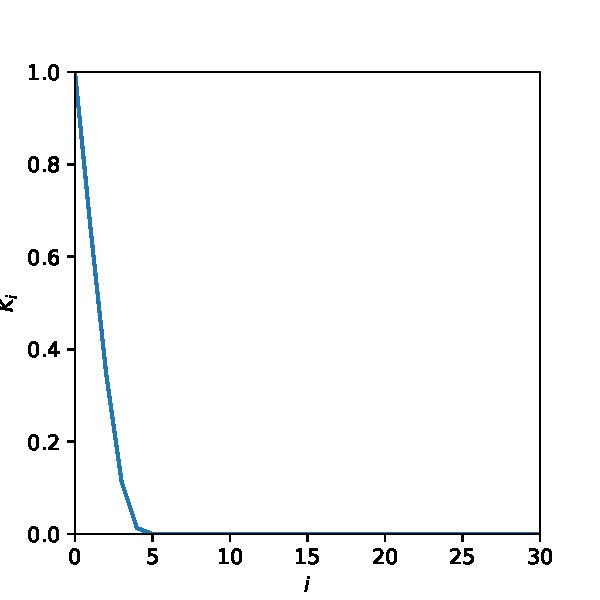
\includegraphics[scale=.7]{./figures/K_series.pdf}
          }
        \end{minipage}%
        \begin{minipage}{.5\linewidth}
          \centering
          \subfloat[free energy increase $g$]{
            \label{:b}
            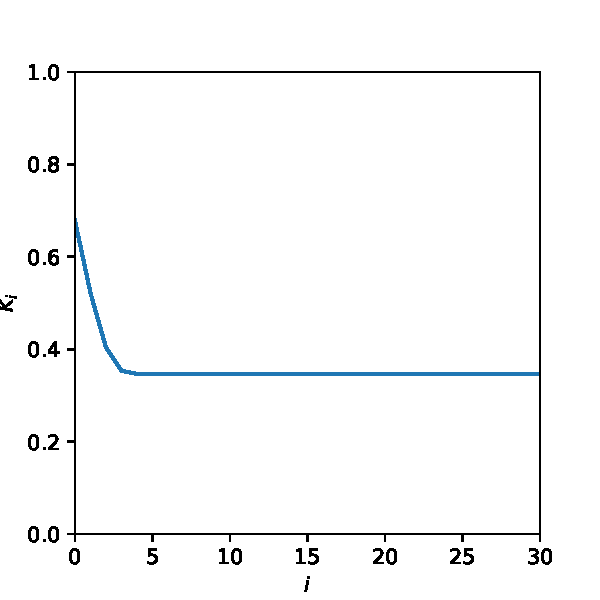
\includegraphics[scale=.7]{./figures/g_series.pdf}
          }
        \end{minipage}
    \end{figure} \ \\


\paragraph{2. Use these results to estimate 
    the dimensionless free energy per spin 
    $f=-\beta F/N$ in fourth order (simply cut 
    the appropriate sum after the term with 
    $g_4$; you can also include the next order
    term, but now by simply using the first 
    term in $g(K)$). Compare to the known 
    exact result for the Ising chain. How good
    is the numerical agreement?
    \textit{(1.5 points)}
}	\ \\
    \\
	Our result by summing the series for $g$:
    \begin{align}
        f
        &=\sum_{i=0}^{4} \frac{g_i}{2^i}
        \approx1.106 \,.
    \end{align}
    Compare to exact result $f=\ln\left(2\cosh(K)\right)=1.127$ for $K=1$.

    \newpage

\end{document}
